\subsection[Ogólny mechanizm działania (Michał Krakowiak)]{Ogólny mechanizm działania}
Podłączenie urządzenia wykonującego do testowanego systemu powinno skutkować rozpoznaniem go jako tzw. Human Interface Device, dalej określanego jako HID. HID to klasa urządzeń korzystających z interfejsu USB do interakcji z człowiekiem, czyli użytkownikiem komputera.
Zazwyczaj wykorzystywane są do pobierania danych wejściowych~\cite{oney}. Interfejs jest powszechnie stosowany przez producentów akcesoriów oraz dobrze udokumentowany w specyfikacji USB~\cite{usbhid}.
Dzięki wysokiej adopcji standardu popularne systemy takie jak Windows, Linux czy macOS są w stanie automatycznie identyfikować nowe urządzenia i korzystać z ich podstawowych funkcjonalności. Często nie ma potrzeby instalacji dedykowanych sterowników.
Ułatwia to pracę pentestera korzystającego z realizowanego systemu. Jeżeli nie planuje on przygotowania niestandardowej funkcjonalności to nie musi implementować i dostarczać własnych sterowników na każdy testowany system komputerowy.
Urządzenia HID komunikują się z komputerem po przez blok danych nazywany raportem. Bity i bajty w nim sformatowane są w sposób określony w deskryptorze raportu.
Listing~\ref{lst:desc} stanowi fragment deskryptora odczytanego bezpośrednio z rzeczywistej klawiatury.
\begin{lstlisting}[language={},label={lst:desc},caption={Przykładowy deskryptor odczytany z istniejącej klawiatury}]
Usage Page (Desktop),                   ; Generic desktop controls (01h)
Usage (Keyboard),                       ; Keyboard (06h, application collection)
Collection (Application),
    Usage Page (Keyboard),              ; Keyboard/keypad (07h)
    Usage Minimum (KB Leftcontrol),     ; Keyboard left control (E0h, dynamic value)
    Usage Maximum (KB Right GUI),       ; Keyboard right GUI (E7h, dynamic value)
    Logical Minimum (0),
    Logical Maximum (1),
    Report Size (1),
    Report Count (8),
    Input (Variable),
    Report Count (1),
    Report Size (8),
    Input (Constant),
    Report Count (3),
    Report Size (1),
    Usage Page (LED),                   ; LEDs (08h)
    Usage Minimum (01h),
    Usage Maximum (03h),
    Output (Variable),
    Report Count (5),
    Report Size (1),
    Output (Constant),
    Report Count (6),
    Report Size (8),
    Logical Minimum (0),
    Logical Maximum (255),
    Usage Page (Keyboard),              ; Keyboard/keypad (07h)
    Usage Minimum (None),               ; No event (00h, selector)
    Usage Maximum (FFh),
    Input,
End Collection
\end{lstlisting}
Każdy deskryptor rozpoczyna się od dyrektywy \textit{Usage Page},
która wskazuje interpretacje kolejnych stałych liczbowych.
Dostępne są tabele zawierające wszystkie możliwe wartości pól deskryptora.
Są one dostarczane przez twórców standardu jako \textit{HID Usage Tables}~\cite{hut}.
Pole \textit{Collection} opisuje zbiór powiązanych ze sobą elementów. W tym przypadku są to raporty: wyjściowy i wejściowy.
Raport wejściowy \textit{(ang. input report)} jest przekazywany do systemu komputerowego i zawiera informację o wciśniętych klawiszach.
Z kolei raport wyjściowy \textit{(ang. output report)} jest przeznaczony dla urządzenia USB i może być wykorzystywany np. do ustawiania jego stanu.
Ważny odnotowania jest fakt, że opisy pól w raportach mogą być wymieszane ze sobą.
Człowiek może mylnie interpretować obecność w sumie 5 dyrektyw \textit{Input} i \textit{Output} jako opis 5 różnych struktur.
W rzeczywistości należy je odczytywać jako przynależność do poszczególnych typów.
Z deskryptora przytoczonego listingu~\ref{lst:desc} można odczytać struktury składające się z:
\begin{itemize}
    \item 8 jednobitowych pól raportu wejściowego, każe przyjmuje wartości od 0 do 1. Poszczególne bity odpowiadają modyfikatorom takim jak np. shift lub alt.
    \item 1 ośmiobitowe pole raportu wejściowego o stałej wartości, to pole nie wpływa na interpretację danych, więc dalszy opis można pominąć
    \item 3 jednobitowe pola raportu wyjściowego, które odpowiadają za modyfikatory diód LED klawiatury (np. wskaźnik caps lock)
    \item 5 jednobitowych pól raportu wyjściowego o stałej wartości, stanowią dopełnienie do pojedyńczego bajtu
    \item 6 ośmiobitowych pól raportu wejściowego o wartościach od 0 do 255, odpowiadają kodom wciśniętych klawiszy
\end{itemize}
Wynikowe struktury ilustruje rysunek~\ref{fig:report}.
%TODO ogarnąć grafikę odpowiadającą deskryptorowi
\begin{figure}[H]
    \centering
    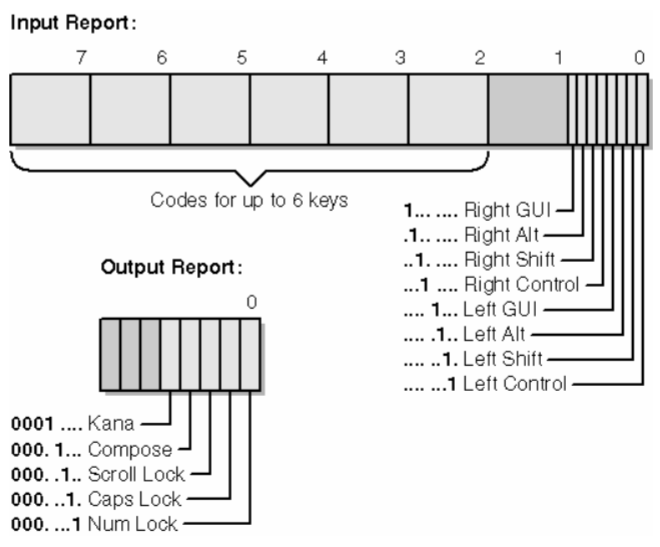
\includegraphics[width=\textwidth]{images/mk02.png}
    \caption{Struktura raportu~\cite{oney}}
    \label{fig:report}
\end{figure}
Implementacja symulowania działania klawiatury będzie polegała na implementacji generowania prawidłowych raportów wejściowych.
Obsługę raportów wejściowe można zignorować. Nie jest ona wymagana do poprawnego działania systemu, ponieważ zapalanie odpowiednich indykatorów nie jest częścią wymagań funkcjonalnych.
Wartości, jakie należy nadać poszczególnym bajtom, aby wskazać wciśnięcie danego klawisza można odczytać z przytoczonego już \textit{HID Usage Tables}. 
Warto mieć na uwadze, że nie ma żadnego powiązania z kodami ASCII. Przykładowo wartość zarówno dla znaków 'a' oraz 'A' to 04h (rozróżnia je odpowiedni modyfikator przesyłany w pierwszym bajcie), podczas gdy w ASCII to odpowiednio 61h i 41h. Obsługa kodu klawisza wysyłane przez urządzenia HID może się różnić w zależności od systemu operacyjnego, np. tylko system MacOS obsługuje kody klawiszy od F13 do F15~\cite{hut}.
